\documentclass{article}
\usepackage{tikz, comment}
\usepackage{pifont}
\usepackage{fontspec}
\usetikzlibrary{arrows, decorations.markings, decorations.pathreplacing}
\begin{comment}
:Title: Not defined yet
:Tags: area using parametric equations,parametric integral formula;area under a curve;average rate of change, arc ;arc length of a curve;moment
:Prob: 0.6201;0.5219;0.4938;0.4848;0.474
:Author: Prof.Hu Ji-shan, HKUST
:Slug: No name yet

Description Here.........
\end{comment}
\begin{document}\centering

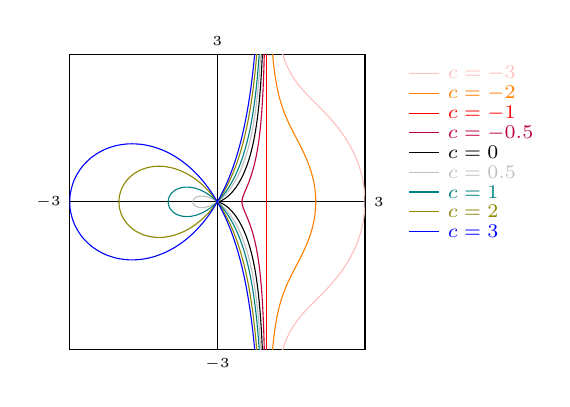
\begin{tikzpicture}[>=latex,xscale=0.375*10/6, yscale=0.375*10/6][font=\sf\small]

%\draw[xstep=1cm,ystep=1cm,color=gray!20] (-2, -2) grid (2, 2);

\draw[] (-3, 0) -- (3, 0);
\draw[] (0, -3) -- (0, 3);

\node[left] at (-3, 0) {\tiny$-3$};
\node[right] at (3, 0) {\tiny$3$};
\node[below] at (0, -3) {\tiny$-3$};
\node[above] at (0, 3) {\tiny$3$};

\draw [pink] (3.5+0.4, {3-1*0.4}) --++(0.6, 0)node[right] {\scriptsize$c=-3$};
\draw [orange] (3.5 +0.4, {3-2*0.4}) --++(0.6, 0)node[right] {\scriptsize$c=-2$};
\draw [red] (3.5 +0.4, {3-3*0.4}) --++(0.6, 0)node[right] {\scriptsize$c=-1$};
\draw [purple] (3.5 +0.4, {3-4*0.4}) --++(0.6, 0)node[right] {\scriptsize$c=-0.5$};
\draw [black] (3.5 +0.4, {3-5*0.4}) --++(0.6, 0)node[right] {\scriptsize$c=0$};
\draw [lightgray] (3.5 +0.4, {3-6*0.4}) --++(0.6, 0)node[right] {\scriptsize$c=0.5$};
\draw [teal] (3.5 +0.4, {3-7*0.4}) --++(0.6, 0)node[right] {\scriptsize$c=1$};
\draw [olive] (3.5 +0.4, {3-8*0.4}) --++(0.6, 0)node[right] {\scriptsize$c=2$};
\draw [blue] (3.5 +0.4, {3-9*0.4}) --++(0.6, 0)node[right] {\scriptsize$c=3$};

\clip[draw] (-3, -3) rectangle (3, 3);

\draw[pink, samples=100, smooth, domain=-5:5, variable=\t]
plot ({((\t)^2-(-3))/((\t)^2+1)}, {(\t)*((\t)^2-(-3))/((\t)^2+1)}); %c=-3

\draw[orange, samples=100, smooth, domain=-5:5, variable=\t]
plot ({((\t)^2-(-2))/((\t)^2+1)}, {(\t)*((\t)^2-(-2))/((\t)^2+1)}); %c=-2

\draw[red, samples=100, smooth, domain=-5:5, variable=\t]
plot ({((\t)^2-(-1))/((\t)^2+1)}, {(\t)*((\t)^2-(-1))/((\t)^2+1)}); %c=-1

\draw[purple, samples=100, smooth, domain=-5:5, variable=\t]
plot ({((\t)^2-(-0.5))/((\t)^2+1)}, {(\t)*((\t)^2-(-0.5))/((\t)^2+1)}); %c=-0.5

\draw[black, samples=100, smooth, domain=-5:5, variable=\t]
plot ({((\t)^2-(0))/((\t)^2+1)}, {(\t)*((\t)^2-(0))/((\t)^2+1)}); %c=0

\draw[lightgray, samples=100, smooth, domain=-5:5, variable=\t]
plot ({((\t)^2-(0.5))/((\t)^2+1)}, {(\t)*((\t)^2-(0.5))/((\t)^2+1)}); %c=0.5

\draw[teal, samples=100, smooth, domain=-5:5, variable=\t]
plot ({((\t)^2-(1))/((\t)^2+1)}, {(\t)*((\t)^2-(1))/((\t)^2+1)}); %c=1

\draw[olive, samples=100, smooth, domain=-5:5, variable=\t]
plot ({((\t)^2-(2))/((\t)^2+1)}, {(\t)*((\t)^2-(2))/((\t)^2+1)}); %c=2

\draw[blue, samples=100, smooth, domain=-5:5, variable=\t]
plot ({((\t)^2-(3))/((\t)^2+1)}, {(\t)*((\t)^2-(3))/((\t)^2+1)}); %c=3

\end{tikzpicture}
\end{document}